% Created by tikzDevice version 0.12.3.1 on 2021-04-14 13:17:10
% !TEX encoding = UTF-8 Unicode
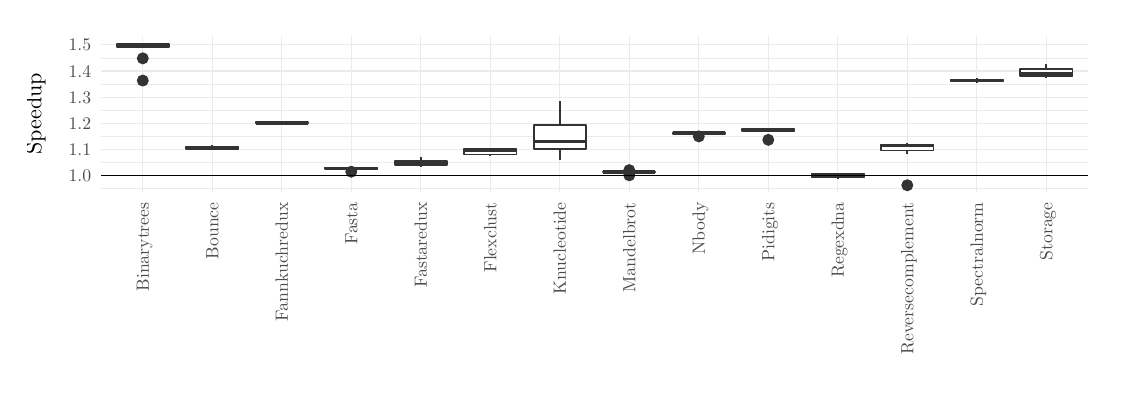
\begin{tikzpicture}[x=1pt,y=1pt]
\definecolor{fillColor}{RGB}{255,255,255}
\path[use as bounding box,fill=fillColor,fill opacity=0.00] (0,0) rectangle (390.26,130.09);
\begin{scope}
\path[clip] ( 26.53, 70.57) rectangle (383.14,127.24);
\definecolor{drawColor}{gray}{0.92}

\path[draw=drawColor,line width= 0.2pt,line join=round] ( 26.53, 71.98) --
	(383.14, 71.98);

\path[draw=drawColor,line width= 0.2pt,line join=round] ( 26.53, 81.42) --
	(383.14, 81.42);

\path[draw=drawColor,line width= 0.2pt,line join=round] ( 26.53, 90.85) --
	(383.14, 90.85);

\path[draw=drawColor,line width= 0.2pt,line join=round] ( 26.53,100.29) --
	(383.14,100.29);

\path[draw=drawColor,line width= 0.2pt,line join=round] ( 26.53,109.72) --
	(383.14,109.72);

\path[draw=drawColor,line width= 0.2pt,line join=round] ( 26.53,119.16) --
	(383.14,119.16);

\path[draw=drawColor,line width= 0.4pt,line join=round] ( 26.53, 76.70) --
	(383.14, 76.70);

\path[draw=drawColor,line width= 0.4pt,line join=round] ( 26.53, 86.14) --
	(383.14, 86.14);

\path[draw=drawColor,line width= 0.4pt,line join=round] ( 26.53, 95.57) --
	(383.14, 95.57);

\path[draw=drawColor,line width= 0.4pt,line join=round] ( 26.53,105.00) --
	(383.14,105.00);

\path[draw=drawColor,line width= 0.4pt,line join=round] ( 26.53,114.44) --
	(383.14,114.44);

\path[draw=drawColor,line width= 0.4pt,line join=round] ( 26.53,123.87) --
	(383.14,123.87);

\path[draw=drawColor,line width= 0.4pt,line join=round] ( 41.60, 70.57) --
	( 41.60,127.24);

\path[draw=drawColor,line width= 0.4pt,line join=round] ( 66.71, 70.57) --
	( 66.71,127.24);

\path[draw=drawColor,line width= 0.4pt,line join=round] ( 91.83, 70.57) --
	( 91.83,127.24);

\path[draw=drawColor,line width= 0.4pt,line join=round] (116.94, 70.57) --
	(116.94,127.24);

\path[draw=drawColor,line width= 0.4pt,line join=round] (142.05, 70.57) --
	(142.05,127.24);

\path[draw=drawColor,line width= 0.4pt,line join=round] (167.17, 70.57) --
	(167.17,127.24);

\path[draw=drawColor,line width= 0.4pt,line join=round] (192.28, 70.57) --
	(192.28,127.24);

\path[draw=drawColor,line width= 0.4pt,line join=round] (217.39, 70.57) --
	(217.39,127.24);

\path[draw=drawColor,line width= 0.4pt,line join=round] (242.51, 70.57) --
	(242.51,127.24);

\path[draw=drawColor,line width= 0.4pt,line join=round] (267.62, 70.57) --
	(267.62,127.24);

\path[draw=drawColor,line width= 0.4pt,line join=round] (292.74, 70.57) --
	(292.74,127.24);

\path[draw=drawColor,line width= 0.4pt,line join=round] (317.85, 70.57) --
	(317.85,127.24);

\path[draw=drawColor,line width= 0.4pt,line join=round] (342.96, 70.57) --
	(342.96,127.24);

\path[draw=drawColor,line width= 0.4pt,line join=round] (368.08, 70.57) --
	(368.08,127.24);
\definecolor{drawColor}{gray}{0.20}
\definecolor{fillColor}{gray}{0.20}

\path[draw=drawColor,line width= 0.4pt,line join=round,line cap=round,fill=fillColor] ( 41.60,119.00) circle (  1.96);

\path[draw=drawColor,line width= 0.4pt,line join=round,line cap=round,fill=fillColor] ( 41.60,110.98) circle (  1.96);

\path[draw=drawColor,line width= 0.6pt,line join=round] ( 41.60,124.07) -- ( 41.60,124.66);

\path[draw=drawColor,line width= 0.6pt,line join=round] ( 41.60,123.05) -- ( 41.60,123.02);
\definecolor{fillColor}{RGB}{255,255,255}

\path[draw=drawColor,line width= 0.6pt,line join=round,line cap=round,fill=fillColor] ( 32.18,124.07) --
	( 32.18,123.05) --
	( 51.02,123.05) --
	( 51.02,124.07) --
	( 32.18,124.07) --
	cycle;

\path[draw=drawColor,line width= 1.1pt,line join=round] ( 32.18,123.28) -- ( 51.02,123.28);

\path[draw=drawColor,line width= 0.6pt,line join=round] ( 66.71, 87.10) -- ( 66.71, 87.62);

\path[draw=drawColor,line width= 0.6pt,line join=round] ( 66.71, 86.23) -- ( 66.71, 85.92);

\path[draw=drawColor,line width= 0.6pt,line join=round,line cap=round,fill=fillColor] ( 57.30, 87.10) --
	( 57.30, 86.23) --
	( 76.13, 86.23) --
	( 76.13, 87.10) --
	( 57.30, 87.10) --
	cycle;

\path[draw=drawColor,line width= 1.1pt,line join=round] ( 57.30, 86.67) -- ( 76.13, 86.67);

\path[draw=drawColor,line width= 0.6pt,line join=round] ( 91.83, 96.08) -- ( 91.83, 96.51);

\path[draw=drawColor,line width= 0.6pt,line join=round] ( 91.83, 95.52) -- ( 91.83, 95.13);

\path[draw=drawColor,line width= 0.6pt,line join=round,line cap=round,fill=fillColor] ( 82.41, 96.08) --
	( 82.41, 95.52) --
	(101.24, 95.52) --
	(101.24, 96.08) --
	( 82.41, 96.08) --
	cycle;

\path[draw=drawColor,line width= 1.1pt,line join=round] ( 82.41, 95.65) -- (101.24, 95.65);
\definecolor{fillColor}{gray}{0.20}

\path[draw=drawColor,line width= 0.4pt,line join=round,line cap=round,fill=fillColor] (116.94, 78.04) circle (  1.96);

\path[draw=drawColor,line width= 0.6pt,line join=round] (116.94, 79.62) -- (116.94, 80.13);

\path[draw=drawColor,line width= 0.6pt,line join=round] (116.94, 79.07) -- (116.94, 78.60);
\definecolor{fillColor}{RGB}{255,255,255}

\path[draw=drawColor,line width= 0.6pt,line join=round,line cap=round,fill=fillColor] (107.52, 79.62) --
	(107.52, 79.07) --
	(126.36, 79.07) --
	(126.36, 79.62) --
	(107.52, 79.62) --
	cycle;

\path[draw=drawColor,line width= 1.1pt,line join=round] (107.52, 79.28) -- (126.36, 79.28);

\path[draw=drawColor,line width= 0.6pt,line join=round] (142.05, 81.94) -- (142.05, 83.46);

\path[draw=drawColor,line width= 0.6pt,line join=round] (142.05, 80.49) -- (142.05, 79.85);

\path[draw=drawColor,line width= 0.6pt,line join=round,line cap=round,fill=fillColor] (132.64, 81.94) --
	(132.64, 80.49) --
	(151.47, 80.49) --
	(151.47, 81.94) --
	(132.64, 81.94) --
	cycle;

\path[draw=drawColor,line width= 1.1pt,line join=round] (132.64, 81.42) -- (151.47, 81.42);

\path[draw=drawColor,line width= 0.6pt,line join=round] (167.17, 86.16) -- (167.17, 86.56);

\path[draw=drawColor,line width= 0.6pt,line join=round] (167.17, 84.31) -- (167.17, 83.69);

\path[draw=drawColor,line width= 0.6pt,line join=round,line cap=round,fill=fillColor] (157.75, 86.16) --
	(157.75, 84.31) --
	(176.59, 84.31) --
	(176.59, 86.16) --
	(157.75, 86.16) --
	cycle;

\path[draw=drawColor,line width= 1.1pt,line join=round] (157.75, 85.66) -- (176.59, 85.66);

\path[draw=drawColor,line width= 0.6pt,line join=round] (192.28, 94.98) -- (192.28,103.56);

\path[draw=drawColor,line width= 0.6pt,line join=round] (192.28, 86.21) -- (192.28, 82.24);

\path[draw=drawColor,line width= 0.6pt,line join=round,line cap=round,fill=fillColor] (182.86, 94.98) --
	(182.86, 86.21) --
	(201.70, 86.21) --
	(201.70, 94.98) --
	(182.86, 94.98) --
	cycle;

\path[draw=drawColor,line width= 1.1pt,line join=round] (182.86, 89.08) -- (201.70, 89.08);
\definecolor{fillColor}{gray}{0.20}

\path[draw=drawColor,line width= 0.4pt,line join=round,line cap=round,fill=fillColor] (217.39, 78.61) circle (  1.96);

\path[draw=drawColor,line width= 0.4pt,line join=round,line cap=round,fill=fillColor] (217.39, 76.74) circle (  1.96);

\path[draw=drawColor,line width= 0.6pt,line join=round] (217.39, 78.09) -- (217.39, 78.13);

\path[draw=drawColor,line width= 0.6pt,line join=round] (217.39, 77.86) -- (217.39, 77.59);
\definecolor{fillColor}{RGB}{255,255,255}

\path[draw=drawColor,line width= 0.6pt,line join=round,line cap=round,fill=fillColor] (207.98, 78.09) --
	(207.98, 77.86) --
	(226.81, 77.86) --
	(226.81, 78.09) --
	(207.98, 78.09) --
	cycle;

\path[draw=drawColor,line width= 1.1pt,line join=round] (207.98, 77.94) -- (226.81, 77.94);
\definecolor{fillColor}{gray}{0.20}

\path[draw=drawColor,line width= 0.4pt,line join=round,line cap=round,fill=fillColor] (242.51, 90.80) circle (  1.96);

\path[draw=drawColor,line width= 0.6pt,line join=round] (242.51, 92.21) -- (242.51, 92.32);

\path[draw=drawColor,line width= 0.6pt,line join=round] (242.51, 91.78) -- (242.51, 91.16);
\definecolor{fillColor}{RGB}{255,255,255}

\path[draw=drawColor,line width= 0.6pt,line join=round,line cap=round,fill=fillColor] (233.09, 92.21) --
	(233.09, 91.78) --
	(251.93, 91.78) --
	(251.93, 92.21) --
	(233.09, 92.21) --
	cycle;

\path[draw=drawColor,line width= 1.1pt,line join=round] (233.09, 92.07) -- (251.93, 92.07);
\definecolor{fillColor}{gray}{0.20}

\path[draw=drawColor,line width= 0.4pt,line join=round,line cap=round,fill=fillColor] (267.62, 89.56) circle (  1.96);

\path[draw=drawColor,line width= 0.6pt,line join=round] (267.62, 93.46) -- (267.62, 93.69);

\path[draw=drawColor,line width= 0.6pt,line join=round] (267.62, 92.73) -- (267.62, 92.57);
\definecolor{fillColor}{RGB}{255,255,255}

\path[draw=drawColor,line width= 0.6pt,line join=round,line cap=round,fill=fillColor] (258.20, 93.46) --
	(258.20, 92.73) --
	(277.04, 92.73) --
	(277.04, 93.46) --
	(258.20, 93.46) --
	cycle;

\path[draw=drawColor,line width= 1.1pt,line join=round] (258.20, 93.29) -- (277.04, 93.29);

\path[draw=drawColor,line width= 0.6pt,line join=round] (292.74, 77.36) -- (292.74, 77.50);

\path[draw=drawColor,line width= 0.6pt,line join=round] (292.74, 75.93) -- (292.74, 75.31);

\path[draw=drawColor,line width= 0.6pt,line join=round,line cap=round,fill=fillColor] (283.32, 77.36) --
	(283.32, 75.93) --
	(302.15, 75.93) --
	(302.15, 77.36) --
	(283.32, 77.36) --
	cycle;

\path[draw=drawColor,line width= 1.1pt,line join=round] (283.32, 76.68) -- (302.15, 76.68);
\definecolor{fillColor}{gray}{0.20}

\path[draw=drawColor,line width= 0.4pt,line join=round,line cap=round,fill=fillColor] (317.85, 73.15) circle (  1.96);

\path[draw=drawColor,line width= 0.6pt,line join=round] (317.85, 87.82) -- (317.85, 88.27);

\path[draw=drawColor,line width= 0.6pt,line join=round] (317.85, 85.75) -- (317.85, 84.30);
\definecolor{fillColor}{RGB}{255,255,255}

\path[draw=drawColor,line width= 0.6pt,line join=round,line cap=round,fill=fillColor] (308.43, 87.82) --
	(308.43, 85.75) --
	(327.27, 85.75) --
	(327.27, 87.82) --
	(308.43, 87.82) --
	cycle;

\path[draw=drawColor,line width= 1.1pt,line join=round] (308.43, 87.41) -- (327.27, 87.41);

\path[draw=drawColor,line width= 0.6pt,line join=round] (342.96,111.40) -- (342.96,111.74);

\path[draw=drawColor,line width= 0.6pt,line join=round] (342.96,110.58) -- (342.96,109.92);

\path[draw=drawColor,line width= 0.6pt,line join=round,line cap=round,fill=fillColor] (333.55,111.40) --
	(333.55,110.58) --
	(352.38,110.58) --
	(352.38,111.40) --
	(333.55,111.40) --
	cycle;

\path[draw=drawColor,line width= 1.1pt,line join=round] (333.55,111.17) -- (352.38,111.17);

\path[draw=drawColor,line width= 0.6pt,line join=round] (368.08,115.10) -- (368.08,116.89);

\path[draw=drawColor,line width= 0.6pt,line join=round] (368.08,112.52) -- (368.08,111.75);

\path[draw=drawColor,line width= 0.6pt,line join=round,line cap=round,fill=fillColor] (358.66,115.10) --
	(358.66,112.52) --
	(377.49,112.52) --
	(377.49,115.10) --
	(358.66,115.10) --
	cycle;

\path[draw=drawColor,line width= 1.1pt,line join=round] (358.66,113.65) -- (377.49,113.65);
\definecolor{drawColor}{RGB}{0,0,0}

\path[draw=drawColor,line width= 0.6pt,line join=round] ( 26.53, 76.70) -- (383.14, 76.70);
\end{scope}
\begin{scope}
\path[clip] (  0.00,  0.00) rectangle (390.26,130.09);
\definecolor{drawColor}{gray}{0.30}

\node[text=drawColor,anchor=base east,inner sep=0pt, outer sep=0pt, scale=  0.64] at ( 22.93, 74.50) {1.0};

\node[text=drawColor,anchor=base east,inner sep=0pt, outer sep=0pt, scale=  0.64] at ( 22.93, 83.93) {1.1};

\node[text=drawColor,anchor=base east,inner sep=0pt, outer sep=0pt, scale=  0.64] at ( 22.93, 93.37) {1.2};

\node[text=drawColor,anchor=base east,inner sep=0pt, outer sep=0pt, scale=  0.64] at ( 22.93,102.80) {1.3};

\node[text=drawColor,anchor=base east,inner sep=0pt, outer sep=0pt, scale=  0.64] at ( 22.93,112.24) {1.4};

\node[text=drawColor,anchor=base east,inner sep=0pt, outer sep=0pt, scale=  0.64] at ( 22.93,121.67) {1.5};
\end{scope}
\begin{scope}
\path[clip] (  0.00,  0.00) rectangle (390.26,130.09);
\definecolor{drawColor}{gray}{0.30}

\node[text=drawColor,rotate= 90.00,anchor=base east,inner sep=0pt, outer sep=0pt, scale=  0.64] at ( 43.80, 66.97) {Binarytrees};

\node[text=drawColor,rotate= 90.00,anchor=base east,inner sep=0pt, outer sep=0pt, scale=  0.64] at ( 68.92, 66.97) {Bounce};

\node[text=drawColor,rotate= 90.00,anchor=base east,inner sep=0pt, outer sep=0pt, scale=  0.64] at ( 94.03, 66.97) {Fannkuchredux};

\node[text=drawColor,rotate= 90.00,anchor=base east,inner sep=0pt, outer sep=0pt, scale=  0.64] at (119.14, 66.97) {Fasta};

\node[text=drawColor,rotate= 90.00,anchor=base east,inner sep=0pt, outer sep=0pt, scale=  0.64] at (144.26, 66.97) {Fastaredux};

\node[text=drawColor,rotate= 90.00,anchor=base east,inner sep=0pt, outer sep=0pt, scale=  0.64] at (169.37, 66.97) {Flexclust};

\node[text=drawColor,rotate= 90.00,anchor=base east,inner sep=0pt, outer sep=0pt, scale=  0.64] at (194.49, 66.97) {Knucleotide};

\node[text=drawColor,rotate= 90.00,anchor=base east,inner sep=0pt, outer sep=0pt, scale=  0.64] at (219.60, 66.97) {Mandelbrot};

\node[text=drawColor,rotate= 90.00,anchor=base east,inner sep=0pt, outer sep=0pt, scale=  0.64] at (244.71, 66.97) {Nbody};

\node[text=drawColor,rotate= 90.00,anchor=base east,inner sep=0pt, outer sep=0pt, scale=  0.64] at (269.83, 66.97) {Pidigits};

\node[text=drawColor,rotate= 90.00,anchor=base east,inner sep=0pt, outer sep=0pt, scale=  0.64] at (294.94, 66.97) {Regexdna};

\node[text=drawColor,rotate= 90.00,anchor=base east,inner sep=0pt, outer sep=0pt, scale=  0.64] at (320.05, 66.97) {Reversecomplement};

\node[text=drawColor,rotate= 90.00,anchor=base east,inner sep=0pt, outer sep=0pt, scale=  0.64] at (345.17, 66.97) {Spectralnorm};

\node[text=drawColor,rotate= 90.00,anchor=base east,inner sep=0pt, outer sep=0pt, scale=  0.64] at (370.28, 66.97) {Storage};
\end{scope}
\begin{scope}
\path[clip] (  0.00,  0.00) rectangle (390.26,130.09);
\definecolor{drawColor}{RGB}{0,0,0}

\node[text=drawColor,rotate= 90.00,anchor=base,inner sep=0pt, outer sep=0pt, scale=  0.80] at (  4.98, 98.91) {Speedup};
\end{scope}
\end{tikzpicture}
